%%&pdflatex
\documentclass[12pt]{report}


\usepackage[utf8]{inputenc}

%docstyle
\usepackage{sectsty}
\sectionfont{\fontsize{13}{15}\selectfont}
\subsectionfont{\fontsize{13}{15}\selectfont}

\usepackage{etoolbox}
\makeatletter
\patchcmd{\@makechapterhead}{\huge}{\fontsize{14}{1}\selectfont}{}{}% for \chapter
\patchcmd{\@makechapterhead}{\Huge}{\fontsize{14}{1}\selectfont}{}{}% for \chapter
\patchcmd{\@makeschapterhead}{\Huge}{\huge}{\fontsize{14}{1}\selectfont}{}{}% for \chapter*
\makeatother

\usepackage{indentfirst} %indent paragraphs
\usepackage[margin=2.5cm]{geometry}
\usepackage{pdfpages}
\usepackage[T1]{fontenc}
\usepackage{mathptmx} %Times New Roman
% \usepackage{fullpage}
% \usepackage{placeins} %for floats position barrier
% \usepackage{float}

%tables
% \usepackage{caption} 
% \usepackage{multirow, supertabular}
% \usepackage{array}
% \usepackage{tabularx}
% \usepackage{makecell}
% \usepackage{hhline}
% \usepackage{changepage}

% \captionsetup[table]{skip=14pt}

%bibliography
% \usepackage{url}
% \bibliographystyle{abbrv}

%graphics
% \usepackage{graphicx}
% \usepackage{subcaption}

\title{Web-Based System for the Extraction of Collocations from Corpora of Polish Texts Equipped with Mechanism for Tunning on Training Data.}
\author{Igor Danielewicz\\ \and Supervisor: dr inż. Michał Przewoźniczek}


%DOCUMENT
\begin{document}
\begin{titlepage}
	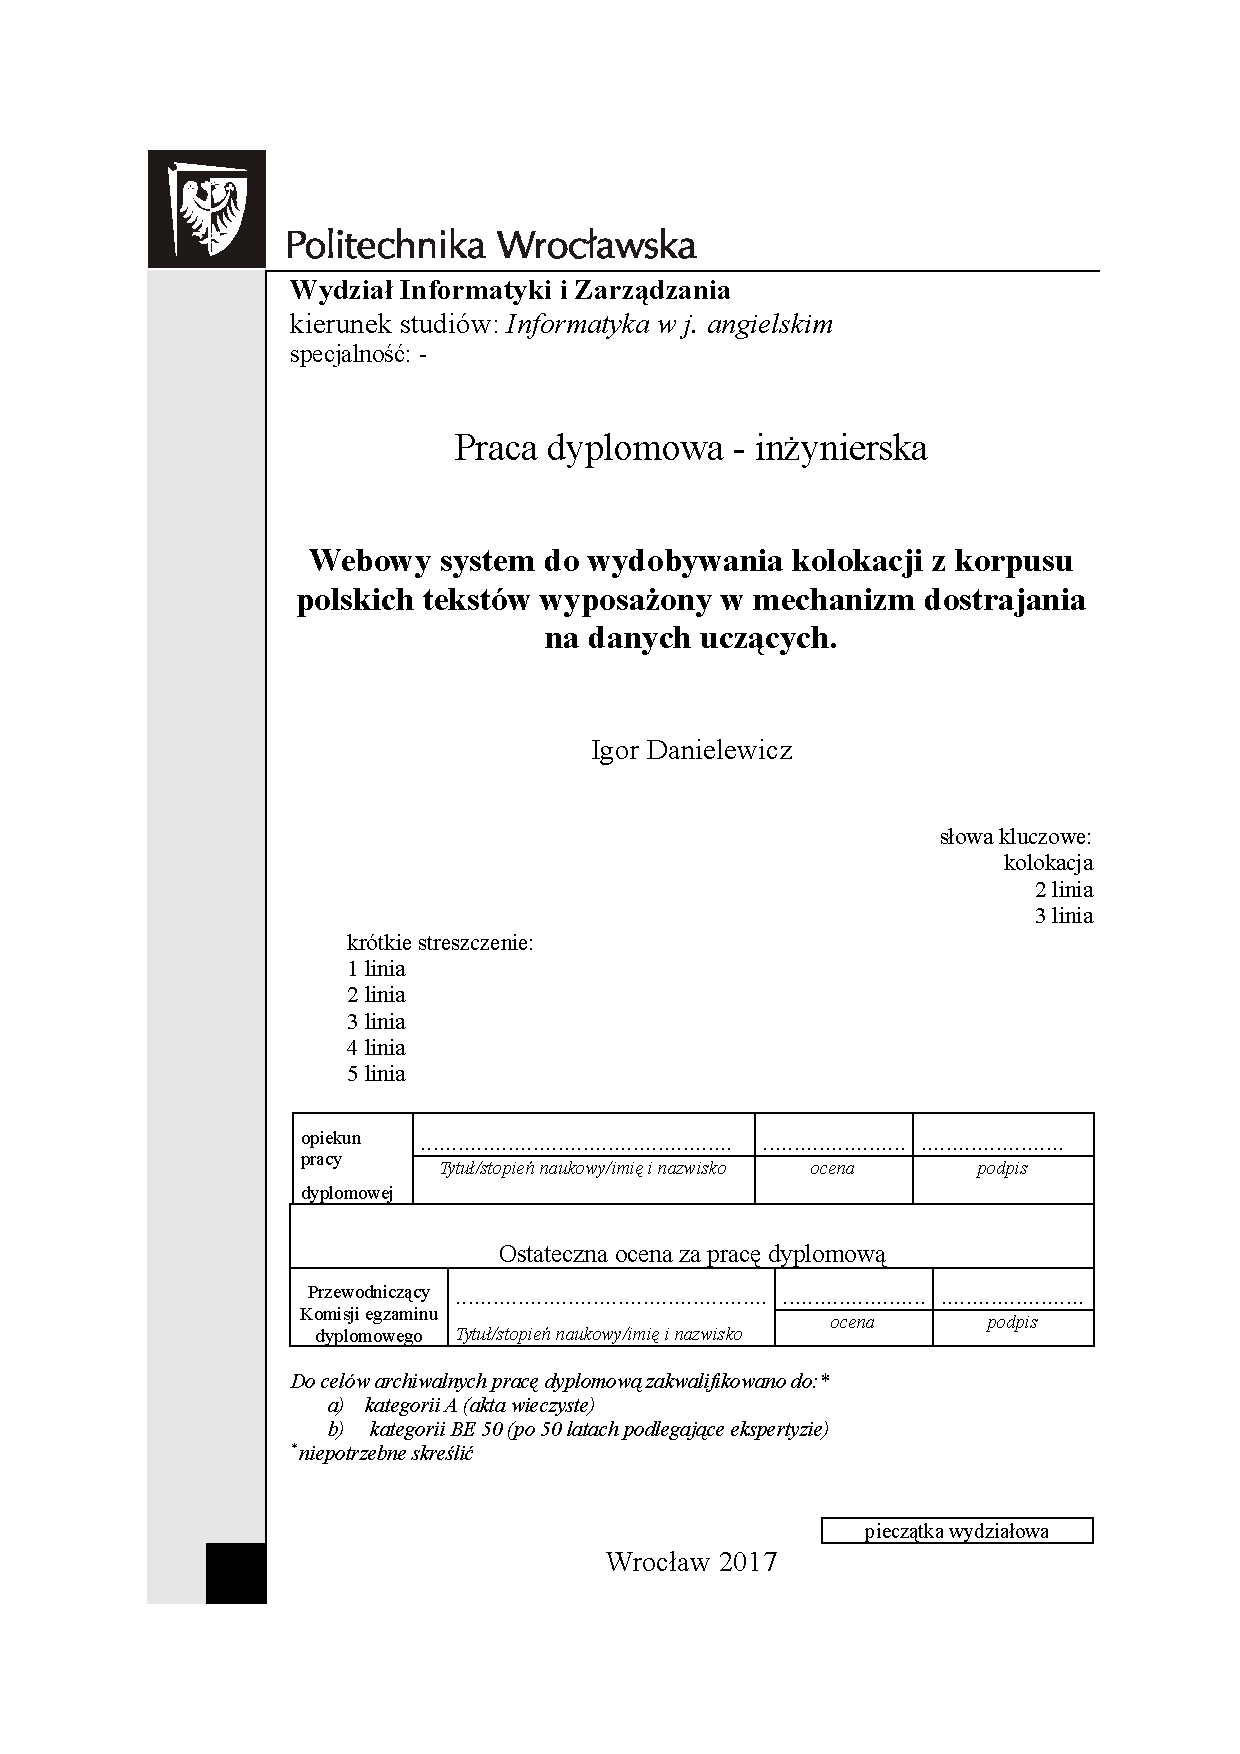
\includepdf[pages={1}]{titlepage.pdf}
\end{titlepage}


\section*{Abstract}
Thesis describe process of improving web based system for extraction of
collocations called MeWeX. At first it characterizes the problem of automatic extraction of collocations 
and introduces the system itself, its structure and functioning. Next chapters present all steps 
which were performed in order to improve quality of the MeWeX, that includes: performing unit tests,
implementing new association measure, implementing new algorithm for tuning
weights and training on new data. Finally it verifies the results achived by the new, 
updated, version of the system comparing it to old results.

\vspace{5em}

\section*{Streszczenie}
Praca opisuje proces ulepszania systemu webowego do ekstrakcji kolokacji, z korpusu tekstów języka polskiego, zwanego MeWeX.
Przedstawia ona problem automatycznej ekstrakcji kolokacji i prezentuje wspomniany system, opisując jego strukturę i 
sposób działania. Kolejne rozdziały przybliżają wszystkie kroki jakie zostały podjęte do polepszenia jakości wyników 
otrzymywanych przez MeWeXa, w tym: wykonanie testów jednostkowych, implementacja nowej miary asocjacyjnej,
implementacja nowego algorytmu do trenowania wektora wag, dostrojenie agregatora miar z użyciem nowego algorytmu 
na nowych danych treningowych. Ostatnim krokiem jest weryfikacja wyników otrzymanych z ulepszonej wersji systemu 
i porównanie ich do poprzednich rezultatów.

\tableofcontents


\chapter{Introduction}

\section{Definition of collocation}


Precise defining collocation is not a simple task. This problem was nicely illustrated by Choueka in Stefan Evert book 
\textit{"Even though any two lexicographers would agree that ’once upon a time’, ’hit the road’ and similar idioms are collocations,
they would most certainly disagree on almost anything else."}
Lexicographers argued over the years on correct defining what collocation is and because of that there is not one fixed definition of collocation  
and in relevant literature we can find many different versions but most of them have one common characteristic, 
collocation is a multiword expression that are syntactically and/or semantically idiomatic. Because this thesis will base on MeWeX system 
it assumes the same definition as in Michał Wendelberger thesis, for which purpose MeWeX was created.
\begin{quote}
    Collocation is a multiword specialistic term or noncompositional general term. 
    It may be both continous or not and both in fixed or flexible order.
    \cite{mgr}
    % Za wyrażenie wielowyrazowe uznawane są wieloelementowe terminy specjalistyczne oraz
    % niekompozycyjne terminy ogólne. Mogą być one zarówno ciągłe, w szyku przemiennym, jak i
    % ustalonym.
\end{quote}
This definition was motivated by similarity to others definitions used by lexicographers and it fits the needs for creating polish MWE "dictionary/lexicon". 

\section{Methods for extraction of collocations} \label{extraction_method}
Automatic extraction of collocations is a very hard task. First of all precise specification of collocation is required.
Method of extraction is dependent on choosen definition of MWE but also on other factors like language. 
Even having precisly specified all conditions it may be performed in many different ways. 
Usually finding MWE is done in three steps. At first candidates for collocation are extracted from the text using some rules and filters, 
which most often base on grammar of given language. Second step is to evaluate quality of the candidates 
using some association measure or more sophisticated algorithms and sorting it according to obtained values. 
Finally collocations are choosen from generated ranking. Method used in MeWeX fits in mentioned above general way, 
more detailed description is included in section \ref{mewex_workflow}.

\section{MeWex}

\subsection{General description}
MeWeX is a system designed for extraction of collocations. It is designed as a set of separate programs 
that preforms consequitive parts of extraction process, but it can be also used as a software library in other projects. 
This design gives huge flexibility, because it allows to run given part many times in different setup, 
or to preprocess large data and save result of every step. This capabilities are very useful in conducting reaserch. 
It is also helpful in natural language processing where often size of data is very large, so possibility 
to preprocess input once and repeating further stages many times with different setup can save a lot of time.

\subsection{Structure of the program}
MeWeX has a lot functionalities, so to preserve clear and maintainable code it has expanded stucture. 
This also simplify further extensions and modifications of the system. Schema of code structure of more important 
or significant for this thesis parts of MeWeX is presented on figure \ref{img_structure}.

\begin{figure}[ht]
	\centering
	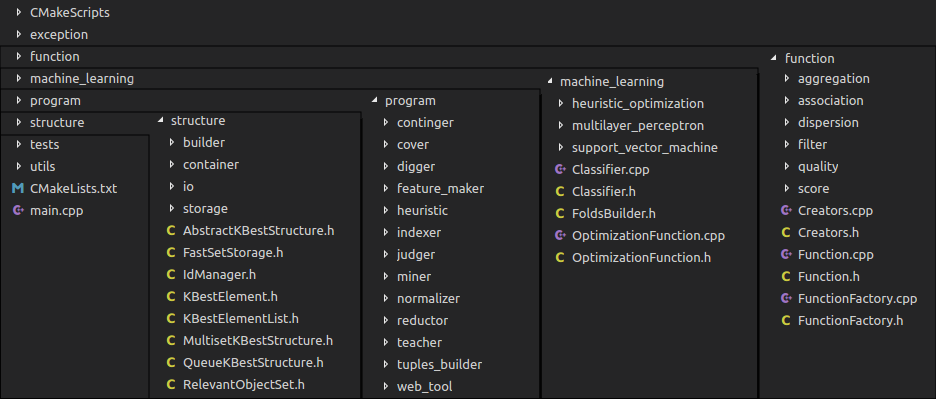
\includegraphics[scale=0.5]{img/mewex_structure.png}
	\caption{Code structure of MeWeX}
	\label{img_structure}
\end{figure}

All functionalities are provided as a set of programs that together creates complete tool for collocation extraction,
verification of the results, tunning weigths, result analysis etc. Below there is a list of all of them together with short description.
\begin{itemize}
    \item \textbf{TuplesBuilder} - Program that reads corpora given as an input and using wccl operators given in input file 
    it creates candidates for collocations.
 
    \item \textbf{Continger} - It creates generators of contingency tables from tuples built by TuplesBuilder.
 
    \item \textbf{Indexer} - This program uses contingency table generators to create set of contingency tables.
 
    \item \textbf{Normalizer} - Program that performs dispersion on contingency tables.
 
    \item \textbf{FeatureMaker} - This program prepares feature vector by evaluating association measures specified at input for each tuple. 
    using output of this program we can train weights for aggregators in reasonable time.
 
    \item \textbf{Heuristic} - It uses given machine learning algorithm to tune weights for association measures. 
    This process is highly adjustable, all parameters for training can be specified in config file.
 
    \item \textbf{Digger} - This program extract collocations basing on given association measures or vector of them. 
    It also provide functionality of extracting encountered forms of collocations.
 
    \item \textbf{Miner} - Program created to perform f-fold cross validation for choosen association measures or classifiers.
    
    \item \textbf{Cover} - It examines coverage of extracted collocations in relations set. It also creates matrix 
    that shows intersection of extracted tuples between relations. It allows to check how many tuples was assigned to more than one relation 
    and which are the most frequent.
 
    \item \textbf{Judger} - This program evaluates results of extracted collocations. It calculates the percentage of correct MWE.
 
    \item \textbf{Reductor} - This program reduces the number of false candidates from set of all tuples created from the text. 
    Ratio of true to false candidates can be specified in parameter.
 
    \item \textbf{WebTool} - Complex tool that performs whole process of extraction at once, starting from plain text 
    it returns list of extracted collocations.
 
    \item \textbf{Teacher} - Program that can be used for training neural network or support vector machine.
 
    
\end{itemize}

\subsection{Workflow of the program} \label{mewex_workflow}
As functionalities of MeWeX are splitted between many separate programs, usually to achive some result several programs must be run in specific order. 
This design, to construct different chains of programs, extends set of possibilities. Some exemplary workflow of the system are described below. 
\\ \textbf{Workflow for evaluation of efficiency of methods for extraction of collocations}
\begin{figure}[ht]
	\centering
	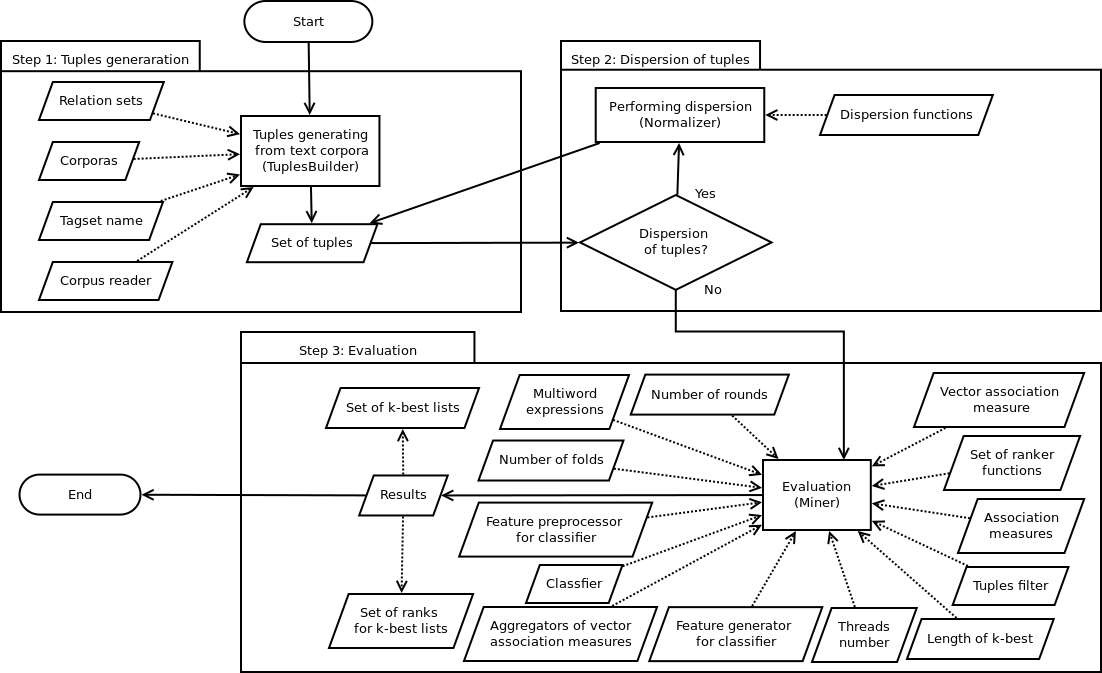
\includegraphics[scale=0.4]{img/mewex_workflow1.png}
	\caption{Examplary workflow}
	\label{img_workflow1}
\end{figure}
\\ Figure \ref{img_workflow1} shows schema of typical path for evaluation of efficiency of given association measure or classifier.
\\ \textbf{Step 1: Tuples generating}\\
First step is to generate tuples from text using WCCL operators, which determine what groups of words are selected for candidates. 
To preform that step program TuplesBuilder is used. It requires list of corpora, corpus reader and name of tagset and 
set of mentioned before wccl operators. Output of this program is CSV file with one tuple per line, consisting information about relation, 
its name, group and size and also all elements of tuple.
\\ \textbf{Step 2: Normalization}\\
Second step is optional and allows modification of information about tuples using one of availble dispersion function. 
It may be useful for processing many corpora of differentiated categories, because it changes frequency distribution of tuples 
favouring less common candidates.
\\ \textbf{Step 3: Evaluation}\\
Final step is to perform f-fold, r-round cross-validation for given dataset. Program accepts as an input many parameters, 
so they are described in table \ref{tbl_workflow1}. After processing it returns 2 sets of files. First type contains k-best list 
of candidates for every fold in every round for every measure and second includes evaluation of those lists. 
Those files should be further analized by the user. 

\begin{table}[t]
    \centering
    % \begin{tabular}{|l|l|}
    \begin{tabular*}{\textwidth}{|l @{\extracolsep{\fill}} l|}
        \hline 
        \textbf{Name of parameter} & \textbf{Description} \\
        \hline
        Tuple storage & Name of the folder with generated tuples \\
        \hline
        Output & Path to the folder were output will be placed \\
        \hline
        Association Measure & Name of association measure to use, \\& this can be specified many times \\
        \hline
        Vector association measure & Text representing vector association measure \\
        \hline
        Aggregator & Aggregator fuction for vector association measure \\
        \hline
        Classifier & Text representing classifier which has to be used \\
        \hline
        Feature generator & Vector association measure which will be used \\& for generating features for classifier \\
        \hline
        Feature preprocessor & Text representing function which has to be used \\& to normalze features for classifier \\
        \hline
        Relevant set & File containing proper MWE, one in line \\
        \hline
        Quality function & Text representing function for evaluation of quality \\& of extracted collocations \\
        \hline
        Tuple filter & Filter that is used to reduce number of tuples \\
        \hline
        Thread number & Maximal number of threads used by program \\
        \hline
        Number of folds & Number of folds for cross-validation \\
        \hline
        Number of rounds & Number of rounds for cross-validation \\
        \hline
    \end{tabular*} 
    \caption{Input parameters for program Miner}
    \label{tbl_workflow1}
\end{table}

\noindent \textbf{Workflow for extraction of collocations}
\\ Figure \ref{img_workflow2} shows schema of typical path for extraction of MWEs using given association measure or classifier.
Steps 1 and 2 are identical as in previous example, so they will not be described again.
\begin{figure}[ht]
	\centering
	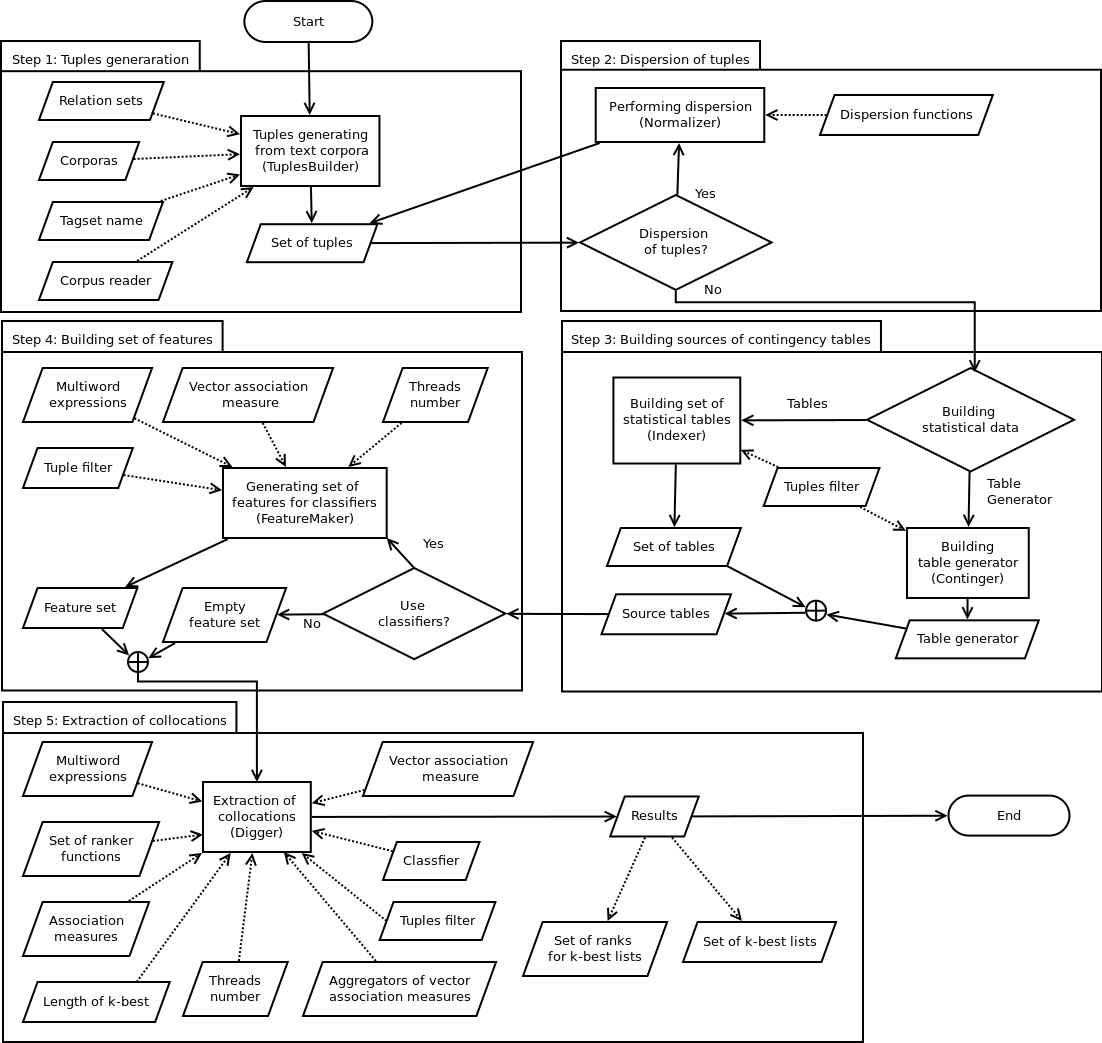
\includegraphics[scale=0.4]{img/mewex_workflow2.png}
	\caption{Examplary workflow}
	\label{img_workflow2}
\end{figure}
\\ \textbf{Step 3: Building contingency table}\\
All measures needs statistical data contained in contingency tables, so they must be generated for further process. 
There are two ways of creating that tables. First is to use Continger, which prepares source of contingency tables, 
this solution uses less memory, but it is more time-consuming. Second way is to use Indexer which generates storage of contingency tables, 
that consumes more memory, but further using those tables requires less time.
\\ \textbf{Step 4: Creating features set}\\
Next step is to prepare features set. This is done be calculating results of all specified association measures for all tuples. 
Those scores will be further used by classifiers or aggregators.
\\ \textbf{Step 5: Extraction}\\
Final step is perform extraction of collocations. This step is performed by program Digger. Input parameters are described 
in table \ref{tbl_workflow1}. Output of this program is similar as in previous case, but this time there are only two files, 
one with k-best list and second includes quality evaluation of this lists, because no cross-validation is performed.

\begin{table}[t]
    \centering
    \begin{tabular*}{\textwidth}{|l @{\extracolsep{\fill}} l|}
        \hline 
        \textbf{Name of parameter} & \textbf{Description} \\
        \hline
        Tuple storage & Name of the folder with generated tuples \\
        \hline
        Contingency tables & Path to file with contingency table source or storage \\
        \hline
        Output & Path to the folder were output will be placed \\
        \hline
        Association Measure & Name of association measure to use, \\& this can be specified many times \\
        \hline
        Vector association measure & Text representing vector association measure \\
        \hline
        Aggregator & Aggregator fuction for vector association measure \\
        \hline
        Classifier & Text representing classifier which has to be used \\
        \hline
        Features set & Path to file with calculated set of features \\
        \hline
        Relevant set & File containing proper MWE, one in line \\
        \hline
        Quality function & Text representing function for evaluation of quality \\& of extracted collocations \\
        \hline
        Tuple filter & Filter that is used to reduce number of tuples \\
        \hline
        Thread number & Maximal number of threads used by program \\
        \hline
    \end{tabular*} 
    \caption{Input parameters for program Digger}
    \label{tbl_workflow2}
\end{table}

\section{Scope of the thesis}

\subsection{General}
Purpose of this thesis is to improve efficiency of the MeWeX. Due to complexity of this system this task 
will consist of few parts listed in sections below.

\subsection{Test association measure functions}
First step is to perform unit test of association measures implementation. Author of the MeWeX did not prepared unit test for this part, 
so there is possibility, that those functions are incorrectly implemented. Errors generated on this stage will propagate in following data process, 
so it can preclude improving further stages. That is why it is important to start with checking correctness of the implementation 
at the beggining.

\subsection{Implement new association measure}
MeWeX was implemented in 2014 and natural language processing is a branch of science developing rapidly nowadays, 
so from that time new association measures may were invented. Task for the author of this tesis is to carefully examine recently written literature 
in search of newly proposed association measures which would be suitable for rating MWE. If some measure will satisfy those condition it should 
be implemented and the last step would be to verify efficiency of that measure.

\subsection{Imlement algorithm for training weigths for vector association measure}
In MeWeX we can evaluate candidates for collocation using not only single association measure, but also aggregated score from more than one measure. 
In that case vector of measures is created and each measure has assigned weigth. Currently in MeWeX there are implemented few simple algorithms 
based on machine learning which trains vector of weigths. For purpose of this thesis new algorithm should be found and implemented.

\subsection{Train classifier on new data}
Mentioned section above algorithms for training weigths needs proper training data. This includes corpora of polish texts and set 
of proper collocations. Michał Wendelberger while working on MeWeX had quite large corpora, but insufficient set of correct MWE limited his results. 
Now in polish Wordnet there is availble much bigger set of collocations. Many of them was gathered with use of MeWeX.
Using new, more copmplete, dataset weigths for aggregators should be retrained in order to obtain better results.

\subsection{Compare new results with previous one}
Last step is to compare results achived by improved version with score that author of MeWeX achieved in his thesis.
To do that, some of the examinations conducted in thesis by Michał Wendelberger will be repeated with new implemented or improved features. 
Only part of experiments will be conducted again, because scope of this thesis does not cover all functionalities offered by MeWeX.
\chapter{Tests}
To ensure correctness fo the results unit testsing should be performed. They cover implementation of all association measures, 
as they were not tested before, so there exists a chance that they are incorrectly written. This should be carefuly examined, 
because errors in that stage will propagate further making improvement of next stages pointless.

\section{Available test frameworks}
There is a lot of unit test frameworks for C++. Thay vary in availble functionalties, in design, differ in their complexity and purpose, 
some of them are heavy-duty, some are ligthweigth and simple. Few exemplary test frameworks are listed below.
\begin{itemize}
    \item \textbf{CppUnit} - test framework that allows testing of C sources as well as C++ with minimal source code modification.
            It was started as a port of JUnit for Windows and ported to Unix. The library is released under the GNU LGP License.
            The framework runs tests in suites. Test result output is sent to a filter, the most basic being a simple pass or fail count printed out, 
            or more advanced filters allowing XML output compatible with continuous integration reporting systems.\footnote{https://en.wikipedia.org/wiki/CppUnit}
    \item \textbf{Boost.Test} - this UTF provides simple writing test cases by using various testing tools. 
            It allows to organize test cases into a test tree. Ease error detection by reporting duties and framework runtime parameters processing.
            More precise description can be found in section \ref{test_boost}.
    \item \textbf{CppUnitLite} - this is a simple C++ testing framework developed by author of the original CppUnit. 
            Unlike some other frameworks, this one is a barebones framework intended to be extended by its users to support their particular needs.
            This approach makes writing individual test easy, one TEST macro which registers the test automatically.\footnote{http://wiki.c2.com/?CppUnitLite}
    \item \textbf{Aeryn} - its design is clean, simple has no dependencies upon other libraries. Although it is primarily intended for unit testing, 
            it is adaptable enough to handle integration testing and can be adapted for most other forms of C++ testing.
            Aeryn requires a modern C++ compiler.\footnote{https://accu.org/index.php/journals/1326}
    \item \textbf{CxxTest} - is a unit testing framework for C++ that is similar in spirit to JUnit, CppUnit, and xUnit. 
            CxxTest is easy to use because it does not require precompiling a CxxTest testing library, 
            it employs no advanced features of C++ (e.g. RTTI) and it supports a very flexible form of test discovery.\footnote{http://cxxtest.com/}
\end{itemize}
From those frameworks Boost.Test has been chosen. There are few reasons why this one was the choice. 
At first Boost library is already used by MeWeX, so using this UTF instead of other does not increase number of dependencies of the project. 
Second reason was that Boost library is the only one known to the author of this thesis, so it was also an advantage. 
Finally its capabilities are sufficient for purpose of this project while use of this framework is simple and easy.

\subsection{Used technology}\label{test_boost}
The Boost Test Library Unit Test Framework gives both a simply to use and flexible way of implementation and organization C++ unit test. 
Writing a unit test module is simple and intuitive for begginers, but framework allows more advanced users to perform complex tests \cite{boost}. 
Test module gives possibility to have many small test cases and organise them into test suites. It also provide a feedback for a long test by 
showing the test progress during its work. It does not require any additional library anf for long term usage users of a unit test framework 
it is able to build it as a standalone library. The Boost.Test keeps track of all passed/failed testing tools assertions, 
provides an ability to check the test progress and generates a result report in several different formats.

\section{Method of testing}
To test association measures at first it was neccesary to prepare contingency tables and additionally for several fuctions additionaly RankerData. 
For purpose of generating that objects set of short CCL was used with content prepared to cover all edge cases in evaluation of tuples scores. 
Text reading, tuples generation and creating contingency table source together with RankerData was performed directly with use of availble functions 
and class instead of using separate program. It was performed only once and stored as a Fixture. Every function was covered by one test case which 
compared result of function with correct result for every tuple in all prepared texts. All test cases were groupped to one test suite.

\section{Result}
Results of unit test showed that several association measures were incorrectly implemented. In some cases error lies in lacking minus like in 
LogLikelihood, so it only reverse the score, but in other cases wrong order of operations like in WOrder makes the result completly miscalculated.
Table \ref{tbl_test} shows the results of performed unit tests, red names indicates incorrect implementation, orange represents function, 
which was properly written, but it uses outcome of faulty measure. In remaining functions no errors were found. 
Last step of this part was to fix those implementations which consisted errors.
\begin{table}[t]
    \centering
    \begin{tabular*}{0.9\textwidth}{l @{\extracolsep{\fill}} l}
        \hline \\
        Dice & \textcolor{red}{LogLikelihood} \\
        \textcolor{red}{WOrder} & SmoothedBigram \\
        TScore & UnigramSubtuples \\
        ZScore & PearsonsChiSquare \\
        Jaccard & ExpectedFrequency \\
        \textcolor{orange}{WTFOrder} & MutualExpectation \\
        Frequency & SpecificCorrelation \\
        OddsRatio & WSpecificCorrelation \\
        Sorgenfrei & InversedExpectedFrequency \\
        \textcolor{red}{ConsonniT1} & SpecificExponentialCorrelation \\
        ConsonniT2 & WSpecificExponentialCorrelation \\
        WChiSquare & FairDispersionPointNormalization \\
        AverageBigram & SpecificFrequencyBiasedMutualDependency \\
        MinimalBigram \\
        \\\hline
    \end{tabular*} 
    \caption{Association functions results}
    \label{tbl_test}
\end{table}
\chapter{New association measure}

Natural Language Processing is developing very quickly nowadays, but extraction of collocations is still quite low advanced field \cite{ramisch}. 
In the recent years a couple of papers and books have been published in this topic, but most of them describes method for extraction of MWE in English 
and since this task is strongly language dependent, polish literature about this subject is much more valuable for this thesis.
In 2016 Polish scientists published paper about their application for polish terminology extraction \cite{termopl}. 
Method that they use for that task is very similar to described in section \ref{extraction_method}. 
Whole extraction is a 3-stage process. At first candidates for terms are selected from text basing on grammar rules. 
Second step is evaluation of candidates using term quality measure and making ranking accordingly to the obtained score. 
Final step is filtering out general terms used in many domains by comparing phrases containing that terms to those obtained from non-domain corpora.
Principle of working is similar to the one used in MeWeX, also definition of terminology used in that paper 
partially cover definition of collocation used in this thesis. The difference is, that in opposition to MWE, term can be a single word, 
also terminology is domain-specific only while collocation can be also noncompositional general expression. 
These discrepancies may be easily walk around by adding some simple constraints and then the same method can be used for extracting MWE. 
First stage of processing is very similar to already implemented, so this can be skipped. Last one filters out general terms, 
which is not desired step in collocation extraction. Middle stage uses quality measure to evaluate candidates and sort them 
accordingly to the obtained score, but TermoPL uses for that purpose C-value measure, which is not implemented in MeWeX. 
Extending available list of association measures by this new function can improve efficiency of the system.

\section{C-Value}
Most significant factor in C-value is frequency of given phrase what is a common practice in association measures. 
Longer tuples are less frequent, so multiplying by logarithm of tuple length reduces that disadvantage. 
The most distinctive part from other measures is subtracting frequencies of all tuples containing given phrase divided by number of those tuples. 
This part decreases score for candidates which occure often in different context.
\clearpage
\[ 
    C{\text -}value(p) = \begin{cases}
        l(p) * (freq(p) - \frac{1}{r(LP)}\sum_{lp \in LP}{freq(lp)}) & \text{if } r(LP) > 0\\
        l(p) * freq(p)            & \text{if } r(LP) = 0\\
    \end{cases}
\]
Where: \\
\(p\)  - phrase \\
\(l(p) = ln(length(p))\) \\
\(LP\)  - set of phrases containing \(p\) \\
\(r(LP)\) - number of elements of \(LP\) \\

This function was modified in relation to the one used in TermoPL. In original measure, function \(l(p) = ln(length(p)) + C\) 
contained also constant, because it was based on assumption that length of \(p\) can be equal to 1. This constant was removed 
from formula as it became redundant for MWE.

\subsection{Motivation}
MeWeX contains many association measure which base on frequency, expected frequency, order, number of relation etc. 
and using vector association measure it can make an advantage of all those features at once. That leads to assumption that adding new measure, 
which values properties not considered before, should increase quality of result. C-value base on frequency and length of phrase, 
but also it takes into account number of different contexts it takes. This property is not covered by any other already implemented function.
Measure W Order is quite similar, but this one checks only number of other relations in which given tuples occurred, 
while C-value also accounts tuples which contains given phrase and measures also frequency.

\clearpage
\subsection{Measure implementation}
Expanded structure and modular architecture of MeWeX made simple further extensions of code. To implement new association 
it was necesary to create new class that inherits class \textit{AssociationFunction}.
\vspace{1em}
\begin{lstlisting}
#include "AssociationFunction.h"

namespace function
{
    namespace association
    {

class Cvalue : public AssociationFunction
{
public:
    virtual AssociationMeasurePtrS copy() const override;

    virtual double rankUsingTable(
        TupleId pTupleId,
        ContingencyTable const& pContingencyTable) const override;

    virtual std::string	name() const override;
};

    }
}
\end{lstlisting}
\vspace{1em}
Then, to make it possible to choose that measure in other modules or programs, name of that function had to be added to the mapping,
that maps name to specific function.
\vspace{1em}
\begin{lstlisting}
Creators::FunctionMapping const AssociationFunctionCreators::MAPPING(
{
    ...

    {"c_value",     &Cvalue},
    {"cval",        &Cvalue},

    ...
});
\end{lstlisting}
\clearpage
And last step was to implement the function itself.
\vspace{1em}
\begin{lstlisting}
double Cvalue::rankUsingTable(
                    TupleId pTupleId, 
                    ContingencyTable const& pContingencyTable) const
{
    double LP = 0.0, LPsum = 0.0;
    for(int i = 1; i < pContingencyTable.size() - 1;i++)
    {
        LPsum += pContingencyTable[i].observed;
        if(pContingencyTable[i].observed > 0)
            LP += 1.0;
    }
    double l = log(pContingencyTable.tupleSize());

    if(LP == 0)
    {
        return (l * pContingencyTable[0].observed);
    }
    else
    {
        return (l * (pContingencyTable[0].observed - (LPsum/LP)));
    }
}
\end{lstlisting}
\clearpage

\subsection{Quality evaluation}
In the figure \ref{img_cval} are presented exemplary results obtained with use of C-value association measure. 
It is hard to manually evaluate quality of all results but in top 50 tuples from k-best list almost all suits the definition of collocation, 
so that is satisfactionary score. More precise evaluation, quality of this measure, method and setup for verification 
is described in chapter \ref{verification}.
\begin{figure}[ht]
    \centering
    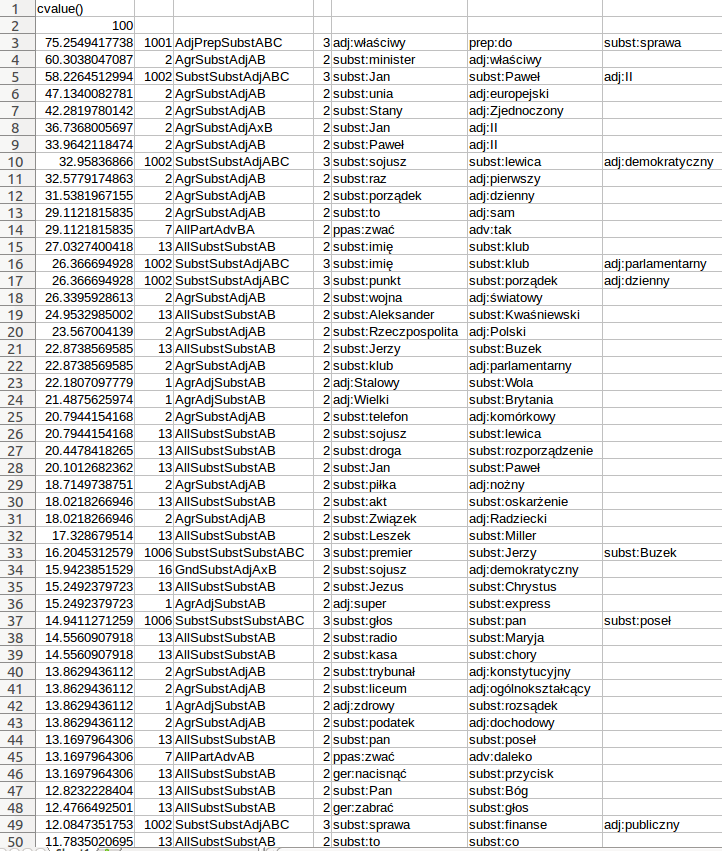
\includegraphics[scale=0.45]{img/cval_res.png}
    \caption{Results obtained with use of C-value association measure}
    \label{img_cval}
\end{figure}

\chapter{Imlement algorithm for training weigths for vector association measure}

MeWeX contains several algorithms which were implemented by Łukasz Kłyk in his \(Optimizer\) and adopted by 
Michał Wendelberger.

TODO

% Wagi rankingów to parametry algorytmu kombinacji, które powinny zostać wyznaczone eks-
% perymentalnie, na przykład poprzez ich optymalizację. Prezentowane oprogramowanie umożli-
% wia wykorzystanie do tego celu pięciu różnych algorytmów heurystycznych i metaheurystycz-
% nych implementacji Łukasza Kłyka [13]. Utworzony przez niego Optimizer został przystoso-
% wany przez autora niniejszej pracy do działania z opisywanym MWeXtractorem. Łukasz Kłyk
% zaimplementował następujące algorytmy w swoim oprogramowaniu:

% Nazwy wspomnianych algorytmów heurystycznych i metaheurystycznych dokładnie określa-
% ją, jakie są to algorytmy, jednak poza dwoma wyjątkami – symulowanym wyżarzaniem i algoryt-
% mem ewolucyjnym. Pierwszy z nich nie precyzuje schematu chłodzenia, ale domyślnie w opro-
% gramowaniu zaimplementowanym przez Łukasza Kłyka stosowana jest funkcja T (k) = 0.3 k
% [13, str. 36]. Przypadek algorytmu ewolucyjnego wymaga dłuższego opisu, ponieważ pojęcie to
% jest znacznie szersze od nazw pozostałych metod.


\begin{itemize}
    \item \textbf{Evolutionary Algorithm} - Description
 
    \item \textbf{Hill Climbing} - Description
 
    \item \textbf{Tabu Search} - Description
 
    \item \textbf{Random Search} - Description
 
    \item \textbf{Simulated Annealing} - Description 
\end{itemize}

\section{Particle Swarm Optimization}\label{pso_def}

Particle Swarm Optimization is an algorithm for optimization of a problem. It tries to improve a candidate solution 
accordingly to a given measure of quality. PSO have population of particles called swarm and solves problem by iteratively moving those particles 
through the search space using formula that involves particle velocity, local best solution and global best solution. 

Algorithm starts with placing all particles in search space choosing random uniformly distributed positions for them and initializing its velocity to 0. 
Then for first particle solution is evaluated, next it assigns its starting position as a local and global best position. 
This step is repeated for all particles in the swarm, but global best position is changed only when new one achieves higher score. 
From that point all steps are performed in a loop till stop condition will not be satisfied. For every paricle, at first 
velocity is updated, then its position is changed by the velocity vector and quality of new position is evaluated. 
If new score is is higher than local or global best, then they are updated accordingly. When algorithm reaches stop conition 
then position of global best solution is returned as a result.
In the figure \ref{pso_flowchart} there is presented flow chart of Particle Swarm Optimization.
\begin{figure}[ht]
    \centering
    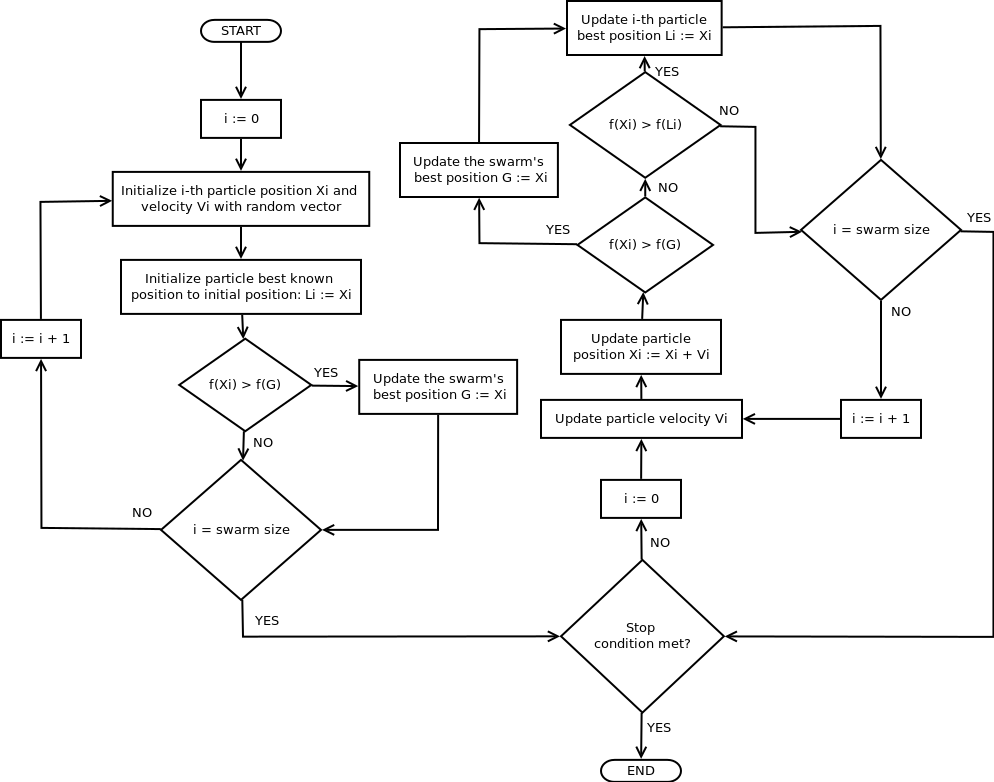
\includegraphics[scale=0.4]{img/pso_flowchart.png}
    \caption{Flow chart of Particle Swarm Optimization}
    \label{pso_flowchart}
\end{figure}

Particles move toward local and global maxima making swarm more dense in surroundings of best known positions. 
That property entail swarm for searching better solutions.
Below there is formula for updating velocity of the particles.
\[ 
    V \gets \omega V + \omega _{p} r _{p} (p - x) + \omega _{g} r _{g} (g - x)
\]
Where: \\
\(V\)  - velocity of given particle, it is vector of size equal to number of dimensions in search space \\
\(r _{p}, r _{g}\) - random numbers from interval \((0,1)\) \\
\(\omega, \omega _{p}, \omega _{g}\) - parameters, chosen by the user, which controls behaviour of the PSO \\
\(x\)  - position of given particle \\
\(p\)  - position of best solution achieved by given particle \\
\(g\)  - position of global best solution achieved by the swarm \\

One of the factor for calculating new velocity is its previous value. Preserving partially old velocity makes particle behavior 
like it would have momentum, smoothing its movement. Particle aims toward global and local best, but force of those both factors is randomized.
New velocity is composed from three vectors and strength of influence for each of them can be adjusted by changing value 
of corresponding \(\omega\) parameter. By modifing those parameters it is possible to control behavior of the swarm, for example 
by reducing momentum or increasing importance of local maxima. TODO

Particle Swarm Optimization is quite simple algorithm, but it can achieve good result. Its simplicity allows easy modification and adjusting 
algorithm for needs of the user. It has three parameters that can influence behavior of the swarm, but their tuning is intuitive. 
Disadvantage of this algorithm is that it has tendency to fall in the local maxima. Next problem is that for high dimensional search spaces 
swarm has to be more populated what greatly increases computational time. 

\subsection{Motivation}
One of the method to increase efficiency of the MeWeX was to improve selection of weigths for aggregators. 
Implementing new algorithm Particle Swarm Optimization was reasonable solution taking into account its simplicity 
connected with good efficacy. Susceptibility on modifications and easy adjustment of parameters make it also a good choice.

\subsection{Implementation}
Expanded structure and modular architecture of MeWeX made simple further extensions of code. Class diagram presented on figure \ref{img_pso_class}
presents the structure of implemented algorithm.
\begin{figure}[ht]
\centering
    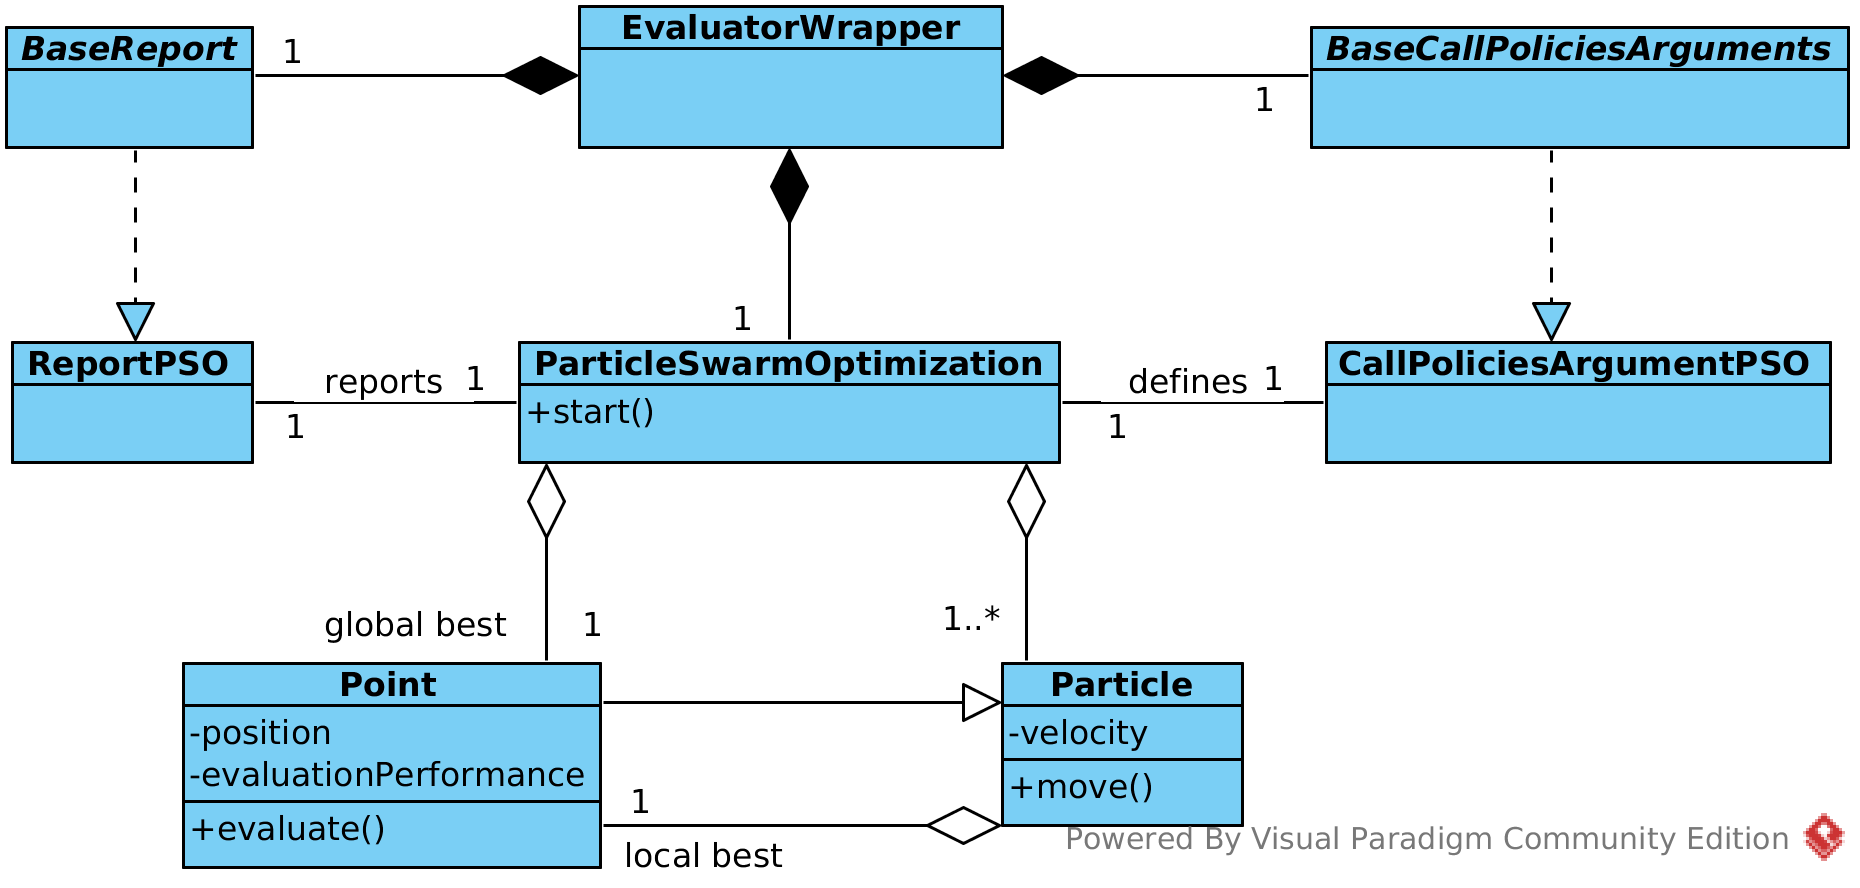
\includegraphics[scale=0.5]{img/pso_class.png}
    \caption{Class diagram of Particle Swarm Optimization}
    \label{img_pso_class}
\end{figure}


To make possible using new algorithm in the same way as already implemented few steps was neccesary to perform.
At first, class \(ParticleSwarmOptimization\) had to be created base on implementation of other machine learning algorithms. 
It does not need to inherit any other class, but it has to be template class, with the same set of template parameters like in other classes. 
Next requirement is that it must define constructor \textit{ParticleSwarmOptimization(const Point\& rStartPoint, Evaluator* pEvaluator, const ArgumentsType\& rArgs)} 
and fuction \(Point\ start()\) which executes whole algorithm and returns best found solution.
Next step was to implement two classes, one which inherits by \(BaseCallPoliciesArguments\) and defines parameters that can be passed by user, 
and second which inherits by \(BaseReport\) and specifies format of creating report of training, which is written to file during algorithm work.
Then, those classes had to be added to \(EvaluatorWrapper\) which is responsible for running chosen algorithm, 
passing arguments from user and creating report. Code below shows modification of that class, where PSO was added.
% \begin{lstlisting}
% class EvaluatorWrapper
% {
% public:

%         ...

%     typedef particle_swarm_optimization::CallPoliciesArgumentsPSO	PSOCallPolicy;

%     enum MethodType
%     {
%         ...

%         PSO,  // Particle Swarm Optimization
%         EMPTY
%     };
%         ...

%     EvaluatorWrapper(
%         EvaluatorPtrR const&	pEvaluator,
%         MethodType              pMethodType,
%         Point const&	        pStartPoint,
%         PSOCallPolicy const& 	pPolicy);

%         ...
    
%     void setParticleSwarmOptimizationPolicy(PSOCallPolicy const& pPolicy);

% private:
%         ...
    
%     PSOCallPolicy mPSOCPA;
% };
% \end{lstlisting}
    
% \begin{lstlisting}
%         ...

% EvaluatorWrapper::EvaluatorWrapper(
%     EvaluatorPtrR const&	pEvaluator,
%     MethodType 			pMethodType,
%     Point const&		pStartPoint,
%     PSOCallPolicy const& 	pPolicy)
% :
%     mMethodType(pMethodType),
%     mStartPoint(pStartPoint),
%     mEvaluator(pEvaluator),
%     mPSOCPA(pPolicy)
% {}

% auto EvaluatorWrapper::parseMethodType(std::string const& pMethod) -> MethodType
% {
%     if(boost::iequals(pMethod, "RS"))
%     {
%         return RS;
%     }    
    
%         ...
        
%     else if(boost::iequals(pMethod, "PSO"))
%     {
%         return PSO;
%     }
%         ...

% void EvaluatorWrapper::setParticleSwarmOptimizationPolicy(PSOCallPolicy const& pPolicy)
% {
%     mPSOCPA = pPolicy;
% }

% auto EvaluatorWrapper::start() -> Point
% {
%         ...

% typedef particle_swarm_optimization::ParticleSwarmOptimization<
%             particle_swarm_optimization::CallPoliciesArgumentsPSO,
%             unsigned int,
%             Step,
%             time_t,
%             Timer,
%             particle_swarm_optimization::ReportPSO> PSOAlgorithm;

%         ...

% switch(mMethodType)
% {
%         ...
        
%     case PSO:
%     {
%         return PSOAlgorithm(mStartPoint, mEvaluator, mPSOCPA).start();
%     }
%     break;

%         ...
% \end{lstlisting}
Last step is to implement algorithm itself, but it needs a class that represents particle and MeWeX machine learning module implements only class \(Point\).
Class \(Particle\) was created by author of this thesis by inheriting class \(Point\), adding velocity vector and best local position and defining 
function \(void\ move(const\ Point\&\ rBest)\).
% \begin{lstlisting}
% void Particle::move(const Point& rBest)
% {
%     double c1 = 1.0, c2 = 0.2, c3 = 0.8;
%     double r1 = Random::random(), r2 = Random::random(), r3 = Random::random();
%     for(int i = 0; i < mVelocity.size(); i++)
%     {
%         double v,mX,rX,cX;
%         auto data = mVelocity[i]->getValueAt(0);
%         mVelocity[i]->getValueAt(0).get(v);
%         mBest->getParameterAt(i).getValueAt(0).get(mX);
%         mParameters[i]->getValueAt(0).get(cX);
%         rBest.getParameterAt(i).getValueAt(0).get(rX);
%         v = (c1 * r1 * v) + (c2 * r2 * (mX - cX)) + (c2 * r2 * (rX - cX));
%         data.set(v);
%         mVelocity[i]->setValueAt(0, data);
%         data.set(cX + v);
%         mParameters[i]->setValueAt(0, data);
%     }
% }
% \end{lstlisting}
Having implemented class \(Particle\) it was possible to write fuction \(Point\ start()\) which executes algorithm. 



\subsection{Improvements}\label{pso_improv}
Initial investigation of algorithm work showed that algorithm improves the score at early stage of work, but then it finds local maximum 
and stops seeking for better solutions. It was caused by the situation where all particles reached the position between 
local and global best solution, so their velocity lowered to values close to zero. Figure \ref{img_pso_imp_plot1} shows the quality of solution 
during algorithm work, where it is visible how swarm has fallen in local maximum and make no progress.
\begin{figure}[ht]
\centering
	\includegraphics[scale=0.5]{img/pso_imp_plot1.png}
	\caption{Plot of PSO algorithm }
	\label{img_pso_imp_plot1}
\end{figure}

To prevent that issue author of this thesis proposed a function which reallocates all particles when algorithm encounter that problem. 
To detect when swarm stopped search, it calculates sum of velocity vector length of all particles. 
If that sum drops below some specified value, function, which places all particle in random position is called. 
\begin{figure}[ht]
	\centering
	\includegraphics[scale=0.5]{img/pso_imp_plot2.png}
	\caption{Plot of PSO algorithm }
	\label{img_pso_imp_plot2}
\end{figure}

Second problem with PSO was that search space had a lot of dimensions, and by reason of long computation time to evaluate single particle solution, 
size of the swarm was limited. This caused that only small part of search space was explored. Solution of that problem, 
proposed by the author of this thesis was to change the distribution of starting positions. Instead of uniform distribution, positions was randomized 
with more problability beeing close to edge. This distibution is presented on figure \ref{img_pso_imp_dist}.

\begin{figure}[ht]
	\centering
	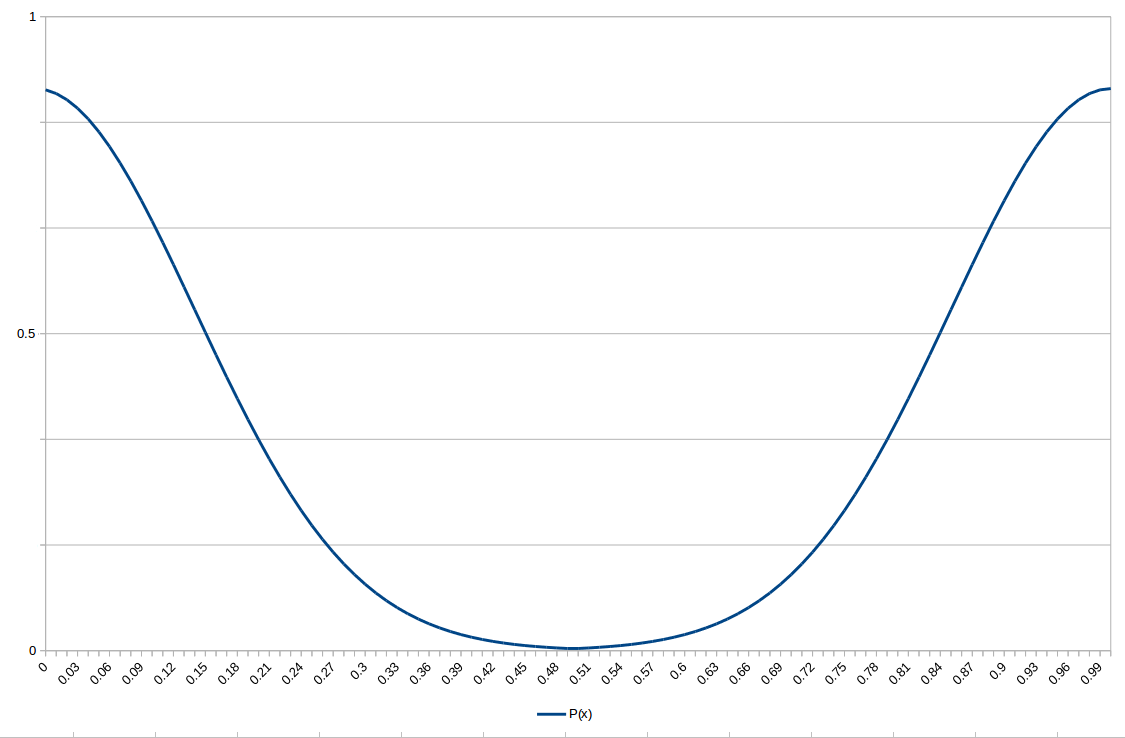
\includegraphics[scale=0.4]{img/pso_dist.png}
	\caption{Probability distribution for selecting particle position}
	\label{img_pso_imp_dist}
\end{figure}

For creation of that probability distribution there was used class, provided by C++11 Standard Library, 
\textit{template< class RealType = double > class normal\_distribution;} which produces random numbers with normal probability
with specified mean and standard deviation. Method, which converts normal distribution to the shown on the plot in the figure \ref{img_pso_imp_dist} 
is shown below.

\begin{lstlisting}
std::normal_distribution<double> Random::normal(0.5, 0.1);
std::mt19937_64 Random::generator(time(nullptr));

double Random::random_inv_normal(void)
{
    double val = normal(generator);
    if(val < 0.5)
    {
        val += 0.5;
        if(val < 0)
            val = 0;
    }
    else
    {
        val -= 0.5;
        if(val > 1)
            val = 1;
    }
    return val;
}
\end{lstlisting}
\chapter{Training classifier}

\section{Dataset}\label{dataset}
During tuning weigths vector 
All association measures base on statistical data, so in order to obtain reliable results large dataset should be provided.
Machine learning algorithms also need vast and differentiated resources to produce satisfactory result.
Below there are described datasets and its sources which was used for purpose of this thesis.

\subsection{Manually Annotated Subcorpus of NKJP}
Manually annotated subcorpus of NKJP is a part of the National Corpus of Polish, which is a initiative of four institutions: 
Institute of Computer Science at the Polish Academy of Sciences, Institute of Polish Language at the Polish Academy of Sciences, 
Polish Scientific Publishers PWN, and the Department of Computational and Corpus Linguistics at the University of Łódź.
It contains one milion tokens and was manually morfosyntactically and semantically annotated by lexicographers. 
Similarly to the main corpus of NKJP it contains text from diverse sources like classic literature, daily newspapers, 
specialist periodicals and journals, transcripts of conversations, and a variety of short-lived and internet texts. 
Manual annotation guarantee correctness of data and it is relatively large what makes it valuable choice for training data.

\subsection{plWordNet Corpus 10.0}

It contains over 4 bilions tokens and it is probably the largest corpus of Polish texts created in controlled way. 
In the article \cite{kgr10} we can find short description of its content: \emph{It consists of IPI PAN Corpus, 
the first annotated corpus of Polish,  National Corpus of Polish, Polish Wikipedia (from 2016), Rzeczpospolita Corpus 
-- corpus of electronic editions of a Polish newspaper from the years 1993-2003, supplemented with text acquired from the Web 
-- only text with small percentage of words unknown to a very comprehensive morphological analyser Morfeusz 2.0 
were included; duplicates were automatically eliminated from the merged corpus.}
Enormous size of this corpus caused computation time to process such amount of information 
long enough to make it impossible to perform tuning weigths and verification of the results on whole corpus. 
That was motivation to utilize only part of that resource. To preserve variety of text, new subcorpus was prepared by randomly picking 
10\% of sentences and dropping rest. Then plain text was annotated by the tager Morphodita\footnote{http://ws.clarin-pl.eu/morphoDiTa.shtml} and stored in CCL format.

\subsection{MWE set from PLWordNet}
Wordnet is a lexically-semantic web, which nodes are lexical units and edges are semantic relations connecting those units.
PLWordNet is the biggest polish wordnet, it was founded by G4.19 Research Group in 2006 and still it is continously developed, 
for now version plWordnet3.1 contains 198000 words, 285000 word's meanings and 670000 semantic relations. Author of this thesis decided to use that resource 
as a source of proper collocations. They were obtained as a set of wccl operators, while MeWeX accepts only MWE listed in file one per line, 
so they had to be preprocessed. This source provided 66853 collocations.

\subsection{Set of relations}
First stage of collocation extraction, selecting candidates, requires set of relations, to reduce number of candidates only to syntactically reasonable. 
These relations has to be in form of WCCL operators. They can specify size of the tuple, part of speech and other properties of phrase element, 
order of tuple or even particular lemma. Set used for purpose of this thesis was taken from resources availble in the MeWeX system. 
At first all relations were used in tuples generation, but examination with use of program \(Cover\) showed that in selected candidates 
there is only 0.44\% of proper collocations. Precise statistics from the output of this program can be found in table \ref{cover_rel_stats}.
Having such large disproportion of positive to negative samples makes training very ineffective. To increase efficacy of learning 
number of incorrect tuples must be reduced. In the table \ref{cover_rel_stats} it is visible, that most of relations have less than 0.05\% 
of positive candidates. Dropping that WCCL operators coverage of proper MWE in generated tuples can be increased to 1.1\%, 
what is still low value, but nevertheless over twice bigger as before. This modification of relation set also greatly shorten computation time 
for all stages following tuples generating, because it decreased number of candidates from 10411380 to 4068265.

\begin{table}[t]
    \centering
    \scriptsize
    \begin{tabular}{|l|r|r|r|}
        \hline 
        \textbf{Relation} & \textbf{MWE} & \textbf{Tuples} & \textbf{Percentage} \\
        \hline
        AdjAdjSubstABC & 1 & 71240 & 0.00140 \\
        AdjAdjSubstABxC & 0 & 22486 & 0.00000 \\
        AdjAdjSubstAxBC & 0 & 117019 & 0.00000 \\
        AdjGenCosAB & 0 & 29 & 0.00000 \\
        AdjGenCosAxB & 0 & 100 & 0.00000 \\
        AdjGenCosBA & 0 & 400 & 0.00000 \\
        AdjGenCosBxA & 0 & 202 & 0.00000 \\
        AdjPrepSubstABC & 30 & 98564 & 0.03044 \\
        AdjPrepSubstABxC & 4 & 73348 & 0.00545 \\
        AdjPrepSubstAxBC & 1 & 99422 & 0.00101 \\
        AdjSubstAdjABC & 31 & 108010 & 0.02870 \\
        AdjSubstAdjABxC & 1 & 119024 & 0.00084 \\
        AdjSubstAdjAxBC & 6 & 78200 & 0.00767 \\
        AdjSubstSubstABC & 27 & 129569 & 0.02084 \\
        AdjSubstSubstABxC & 2 & 198777 & 0.00101 \\
        AdjSubstSubstAxBC & 2 & 79647 & 0.00251 \\
        AgrAdjSubstAB & 2099 & 358130 & 0.58610 \\
        AgrAdjSubstAxB & 437 & 78905 & 0.55383 \\
        AgrAdjSubstBA & 4832 & 183497 & 2.63329 \\
        AgrAdjSubstBxA & 306 & 70984 & 0.43108 \\
        AgrSubstAdjAB & 8159 & 183497 & 4.44639 \\
        AgrSubstAdjAxB & 388 & 70984 & 0.54660 \\
        AgrSubstAdjBA & 1945 & 358130 & 0.54310 \\
        AgrSubstAdjBxA & 606 & 78905 & 0.76801 \\
        AllAdvPartAB & 7 & 22417 & 0.03123 \\
        AllAdvPartAxB & 0 & 14175 & 0.00000 \\
        AllAdvPartBA & 0 & 11715 & 0.00000 \\
        AllAdvPartBxA & 0 & 10347 & 0.00000 \\
        AllBurkSubstAB & 0 & 1426 & 0.00000 \\
        AllBurkSubstAxB & 0 & 981 & 0.00000 \\
        AllBurkSubstBA & 0 & 1402 & 0.00000 \\
        AllBurkSubstBxA & 0 & 1402 & 0.00000 \\
        AllGerQubAB & 292 & 1912 & 15.27197 \\
        AllGerQubAxB & 16 & 2021 & 0.79169 \\
        AllGerQubBA & 56 & 2619 & 2.13822 \\
        AllGerQubBxA & 116 & 4546 & 2.55169 \\
        AllNumSubstAB & 15 & 74696 & 0.02008 \\
        AllNumSubstAxB & 8 & 79706 & 0.01004 \\
        AllNumSubstBA & 4 & 72716 & 0.00550 \\
        AllNumSubstBxA & 6 & 115139 & 0.00521 \\
        AllPartAdvAB & 227 & 11715 & 1.93769 \\
        AllPartAdvAxB & 16 & 10347 & 0.15463 \\
        AllPartAdvBA & 51 & 22417 & 0.22751 \\
        AllPartAdvBxA & 84 & 14175 & 0.59259 \\
        AllQubGerAB & 0 & 2619 & 0.00000 \\
        AllQubGerAxB & 0 & 4546 & 0.00000 \\
        AllQubGerBA & 0 & 1912 & 0.00000 \\
        AllQubGerBxA & 0 & 2021 & 0.00000 \\
        AllSiebieSubstAB & 0 & 2826 & 0.00000 \\
        AllSiebieSubstAxB & 0 & 3303 & 0.00000 \\
        AllSiebieSubstBA & 0 & 1072 & 0.00000 \\
        AllSiebieSubstBxA & 0 & 2465 & 0.00000 \\
        AllSubstBurkAB & 1 & 1402 & 0.07133 \\
        AllSubstBurkAxB & 1 & 1402 & 0.07133 \\
        AllSubstBurkBA & 0 & 1426 & 0.00000 \\
        AllSubstBurkBxA & 0 & 981 & 0.00000 \\
        AllSubstNumAB & 2 & 72716 & 0.00275 \\
        \end{tabular}
        \quad
        \begin{tabular}{|l|r|r| r|}
        \hline 
        \textbf{Relation} & \textbf{MWE} & \textbf{Tuples} & \textbf{Percentage} \\
        \hline
        AllSubstNumAxB & 1 & 115139 & 0.00087 \\
        AllSubstNumBA & 0 & 74696 & 0.00000 \\
        AllSubstNumBxA & 0 & 79706 & 0.00000 \\
        AllSubstSiebieAB & 4 & 1072 & 0.37313 \\
        AllSubstSiebieAxB & 1 & 2465 & 0.04057 \\
        AllSubstSiebieBA & 1 & 2826 & 0.03539 \\
        AllSubstSiebieBxA & 1 & 3303 & 0.03028 \\
        AllSubstSubstAB & 2410 & 931272 & 0.25879 \\
        AllSubstSubstAxB & 588 & 1388050 & 0.04236 \\
        AllSubstSubstBA & 569 & 931272 & 0.06110 \\
        AllSubstSubstBxA & 1011 & 1388050 & 0.07284 \\
        AllVerbSiebieAB & 9050 & 11393 & 79.43474 \\
        AllVerbSiebieAxB & 2339 & 3526 & 66.33579 \\
        AllVerbSiebieBA & 6233 & 8839 & 70.51703 \\
        AllVerbSiebieBxA & 3943 & 6211 & 63.48414 \\
        CosAdjGenAB & 1 & 400 & 0.25000 \\
        CosAdjGenAxB & 0 & 202 & 0.00000 \\
        CosAdjGenBA & 0 & 29 & 0.00000 \\
        CosAdjGenBxA & 0 & 100 & 0.00000 \\
        GndAdjSubstAB & 21 & 3896 & 0.53901 \\
        GndAdjSubstAxB & 71 & 14057 & 0.50509 \\
        GndAdjSubstBA & 51 & 7862 & 0.64869 \\
        GndAdjSubstBxA & 49 & 16888 & 0.29015 \\
        GndSubstAdjAB & 70 & 7854 & 0.89127 \\
        GndSubstAdjAxB & 55 & 16888 & 0.32568 \\
        GndSubstAdjBA & 19 & 3886 & 0.48893 \\
        GndSubstAdjBxA & 96 & 14057 & 0.68293 \\
        Ppron3GenSubstAB & 1 & 8764 & 0.01141 \\
        Ppron3GenSubstAxB & 0 & 6563 & 0.00000 \\
        Ppron3GenSubstBA & 0 & 4613 & 0.00000 \\
        Ppron3GenSubstBxA & 0 & 7406 & 0.00000 \\
        SubstAdjAdjABC & 13 & 32151 & 0.04043 \\
        SubstAdjAdjABxC & 0 & 91908 & 0.00000 \\
        SubstAdjAdjAxBC & 0 & 25040 & 0.00000 \\
        SubstAdjSubstABC & 44 & 156730 & 0.02807 \\
        SubstAdjSubstABxC & 2 & 151333 & 0.00132 \\
        SubstAdjSubstAxBC & 8 & 209355 & 0.00382 \\
        SubstAdvAdjABC & 4 & 13318 & 0.03003 \\
        SubstAdvAdjABxC & 11 & 8651 & 0.12715 \\
        SubstAdvAdjAxBC & 1 & 23663 & 0.00423 \\
        SubstConjSubstABC & 20 & 81567 & 0.02452 \\
        SubstConjSubstABxC & 7 & 57989 & 0.01207 \\
        SubstConjSubstAxBC & 7 & 53419 & 0.01310 \\
        SubstPpron3GenAB & 0 & 4613 & 0.00000 \\
        SubstPpron3GenAxB & 0 & 7406 & 0.00000 \\
        SubstPpron3GenBA & 0 & 8764 & 0.00000 \\
        SubstPpron3GenBxA & 0 & 6563 & 0.00000 \\
        SubstPrepSubstABC & 120 & 221630 & 0.05414 \\
        SubstPrepSubstABxC & 12 & 143286 & 0.00837 \\
        SubstPrepSubstAxBC & 19 & 183775 & 0.01034 \\
        SubstSubstAdjABC & 46 & 98007 & 0.04694 \\
        SubstSubstAdjABxC & 0 & 76129 & 0.00000 \\
        SubstSubstAdjAxBC & 8 & 147898 & 0.00541 \\
        SubstSubstSubstABC & 13 & 88445 & 0.01470 \\
        SubstSubstSubstABxC & 2 & 149396 & 0.00134 \\
        SubstSubstSubstAxBC & 2 & 155425 & 0.00129 \\
        \hline
        Sum & 46703 & 10411380 & 0.44857 \\
        \hline
    \end{tabular} 
    \caption{Coverage of proper collocations from plWordNet per relation in tuples extracted from plWordNet Corpus 10.0 and Manually Annotated Subcorpus of NKJP}
    \label{cover_rel_stats}
\end{table}

\section{Methods used for training}
To train vector of weigths PSO algorithm with modifications described in section \ref{pso_improv} was used. 
Dataset used for learning was both Manually Annotated Subcorpus of NKJP and plWordNet Corpus 10.0. Tuples were generated using reduced set of relations
to increase its efficiency and shorten computation time.

To select proper size of the swarm, short research was conducted on NKJP Subcorpus only, to analyze influence of the number of particles on 
algortihm efficacy. Test was carried out for sizes: 5, 10, 20, 40 and accordingly 4000, 2000, 1000, 500 iterations, 
to preserve the same number of particle evaluations and as a result the same computation time.
Also parameters \(\omega, \omega _l, \omega _g\), were choosen in similar way, by training on small data, with different configurations, 
to select the best found set of values.

Final values that were choosen for training were: \\
\[
\omega = 1.0, \quad
\omega _l = 0.2, \quad
\omega _g = 0.8, \quad
swarm\_size = 40
\]

Measure of quality, that were used as a target for an optimization is Average Precision. It is precisely described in section \ref{ap_desc}.

\section{Results}
Figure \ref{pso_train} presents to process of training showing value of best achieved Average precision value for given iteration.
From the beggining ut to 300 iteration aggregator achieves average score, comparable to aquired by other association measures. 
Next iterations bring vast improvement, quality of the result increases quickly till 1250 iteration, where it reaches the maximum 
obtained by this algorithm. Final returned value of Average Precision is 0.673891.


\begin{figure}[ht]
    \centering
    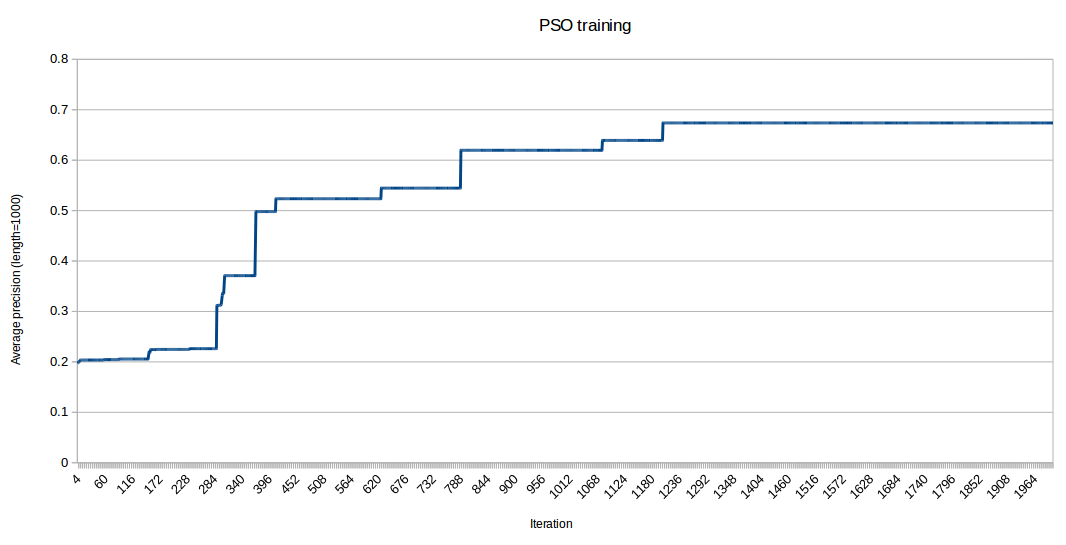
\includegraphics[scale=0.45]{img/pso_train.png}
    \caption{Flow chart of Particle Swarm Optimization}
    \label{pso_train}
\end{figure}
\chapter{Verification of the result} \label{verification}

\section{Methods of results verification}
Final stage of this thesis is to verify quality of newly implemented features. Results were measured with use of Miner program. 
It performs f-fold, r-round cross validation to evaluate given association measure or aggregator. Features which will be aim of 
this verification are C-value association measure and aggregated set of measures with weigths trained by Particle Sworm Optimization. 
Same examination were conducted also for previously implemented measures to compare results. As a final score average from each round 
and each fold of given validation were taken.

\section{Setup for verification}
Verification was performed with use of the datased described in section \ref{dataset}. Association measures listed below 
were used as a reference.
\begin{itemize}
    \setlength\itemsep{0em}
    \item Mutual Expectation
    \item Specific Frequency Biased Mutual Dependency
    \item Tscore
    \item Loglikelihood
    \item Jaccard
    \item Sorgenfrei
    \item Unigram Subtuples
    \item Specific Exponential Correlation with parameter equal to 3,8
    \item W Specific Exponential Correlation with parameter equal to 1,15
    \item W Order
    \item W Term Frequency Order
\end{itemize}

TODO


\section{Results}

TODO
\chapter{Conclusions}

\section{Conclusions}

\section{Further development}


% Shared library available in C++ and package for Python offer same method with similar syntax - method Lemmatize with parameters :\begin{itemize}
% \item inflected phrase
% \item base form of words space-separated
% \item tags of words space-separated
% \item boolean values if the words of phrase should be space-separated
% \item phrase category
% \end{itemize}
% Command-line tool takes tsv file as an input. Each line consist of proper lemma of a phrase, an inflected phrase, base forms of words from the phrase, tags of each word, boolean values if there should be space after each word and a category of a phrase e.g.
        
% \begin{figure}[ht]
% 	\centering
% 	\includegraphics[scale=0.7]{img/karina.jpg}
% 	\caption{Lemmatization Module Input}
% 	%\label{polem_input}
% \end{figure}
        
% Evaluation is based on comparing the proper lemma that was given at input to the result of the lemmatization. Output of the module is also a tsv file with effectiveness of the lemmatization calculated. Each line consists of a boolean value if the lemmatization of the phrase was conducted successfully, inflected phrase, proper lemma of the phrase, category, method that was used to lemmatize given phrase, base form of words in phrase and tags e.g.
        
% \begin{figure}[ht]
% 	%\includegraphics[scale=0.53]{karina.jpg}
% 	\caption{Lemmatization Module Output}
% 	%\label{polem_Output}
% \end{figure}
% At the end of the file the summary of the lemmatization is given concerning the method of lemmatization and concerning the category of phrases. Each method or category is listed with an amount of phrases successfully and unsuccessfully lemmatized, effectiveness and coverage of all phrases by given method or category e.g.
% \begin{figure}[h]
% 	\centering
% 	%\includegraphics[scale=0.7]{karina.jpg}
% 	\caption{Lemmatization Module Output Table}
% 	%\label{polem_output_table}
% \end{figure}

        
% MorfGeo Lemmatizer is another dictionary lemmatizer however file that it uses as dictionary is a list of inflected geological names and locations with their lemmas. NamLivPerson lemmatizer is partial dictionary and partial rule lemmatizer as it uses both dictionary and rules to generate or find lemmas. Dictionary that it also taken from the Nelexicon tool however it consists only of phrases related to and of human full names. Rules for inflection for NamLivPerson are in a form of list with tag of an inflected phrase, ending of an inflected phrase, ending of lemma of the phrase and numerical value that represents frequency of given ending occurring in texts. NamLoc lemmatizer uses only inflection rules to generate lemmas. Rules are in identical form as in NamLivPerson lemmatizer, the only difference between NamLoc and NamLivPerson rule-based part is the category of phrases and dictionary file. Rule Lemmatizer uses rules developed by Ph.D. Marczinczuk and described in "Lemmatization of Multi-word Common Noun Phrases and Named Entities in Polish" paper. //TODO CHANGE AFOREMENTIONED SENTENCE// Rules are in a form of XML DOM file and consists of constraints and transformations. Constraints are encoded using WCCL formalism. Sample rule : 
        
% After entering values, process goes into Nelexicon Lemmatizer part. Dictionary file is searched for lemma for given phrase. If lemma is found the process returns result otherwise process proceeds to MorfGeo Lemmatizer and searches the dictionary file for lemma. When lemma is not found and category of the phrase matches person's name category process starts NamLivPerson Lemmatizer and searches its dictionary file and in case lemma is still not found inflection rules are applied in such manner, that if tag and ending of a word fits the rule, the ending of a lemma from the rule with highest occurrence value is taken and lemma is generated by replacing word's ending with ending from the rule. Phrases are dismembered into words before searching for fitting rule. Lemma is found when there is a rule for every word in a phrase. When taking into consideration the occurrence values, only rules with values higher then certain value are used. If lemma is not found and category of the phrase matches location, NamLoc Lemmatizer is started. For every word in phrase rules of lemmatizer are searched for in same manner that in NamLivPerson rule-based part.  //TODO 
% \section{Evaluation()MORELIKE IMPLEMENTATION }
% //write bout files and result 
% \chapter{Keyword extraction module}
% \chapter{Description of the system as a whole}
% System consists of keyword extractor and lemmatization module. Lemmatization module was added to default process of the extractor.
% \chapter{Implementation}
% \chapter{Summary}
		
% %BIBLIOGRAPHY
% \addcontentsline{toc}{chapter}{List of tables}
% \listoftables
% \addcontentsline{toc}{chapter}{List of figures}
% \listoffigures
% \addcontentsline{toc}{chapter}{Bibliography}
% % 			\bibliography{bibliography.bbl}
% % 			\bibliography{mybib}{}
% \nocite{*}
% %             \bibliographystyle{plain}
% \bibliography{main.bib}
\end{document}
